\documentclass[conference]{IEEEtran}
\usepackage{amsmath,amssymb}
\usepackage{graphicx}
\usepackage{booktabs}
\usepackage{xcolor}
\usepackage{tikz}
\usetikzlibrary{arrows.meta,positioning}
\usepackage{pgfplots}
\pgfplotsset{compat=1.17}
\usepackage[hidelinks]{hyperref}
\newcommand{\code}[1]{\texttt{#1}}
\graphicspath{{../figures/}}

\begin{document}

\title{Aitachi-Hand: An Open 17-DOF Dexterous-Hand Platform and a Controlled\\
Study of Proximal Policy Optimization Improvements for Gesture Control}

\author{\IEEEauthorblockN{Aitachi}
\IEEEauthorblockA{Aitachi-Hand Project\\
github.com/aitachi/Aitachi-Hand}}

\maketitle

\begin{abstract}
We present \textbf{Aitachi-Hand}, an end-to-end open platform that couples the
CC-BY-4.0 ORCA Hand v2 (17 DOF, tendon-driven, Feetech HLS bus servos) with a
fully documented calibration--simulation--control stack, and use it to run a
controlled comparison of reinforcement-learning methods on two dexterous
gesture tasks: (i) \emph{collision-free free posing}, where five fingers must
reach arbitrary poses on the natural-pose manifold without self-collision, and
(ii) \emph{rapid gesture sequencing}, a chained V$\to$OK$\to$OPEN task with
per-phase geometric acceptance. Building on a numerically validated residual
action design that makes the zero policy a solvable direct baseline, we
evaluate three algorithm families---PPO, TD3, and SAC---and six published
PPO-centric improvements (TR-PPO-RB rollback, ESPO early stopping, PPG phasic
updates, ExO-PPO smooth off-policy surrogates, potential-based reward shaping,
and RND intrinsic motivation) under a fixed budget (150k environment steps,
three seeds, shared 256$\times$256 networks, fixed 25-seed deterministic
evaluation). We release the hardware mapping tables (17 axes, measured
min/center/max), the servo protocol appendix, both MuJoCo environments, all
algorithm implementations with their deviations from the original papers
disclosed, 12 comparison figures, and a four-language reproducible experiment
report.
\end{abstract}

\begin{IEEEkeywords}
dexterous hand, reinforcement learning, proximal policy optimization,
reward shaping, tendon-driven actuation, MuJoCo, sim-to-real
\end{IEEEkeywords}

\section{Introduction}
Dexterous hands concentrate the hardest properties of robot learning---high
dimensionality, nonconvex self-collision constraints, and costly real-world
trials---into a cheap, desk-scale package. Open hardware such as the ORCA
Hand~\cite{orca} removes the mechanical barrier; open simulators remove the
software barrier. What remains scarce is a \emph{connected} artifact: measured
servo calibration tied to simulation joints, safety-guarded low-level control
tied to trained policies, and algorithm comparisons tied to one fixed
protocol rather than one paper's tuning budget.

Aitachi-Hand contributes exactly this connection:
\begin{enumerate}
\item a measured 17-axis mapping from Feetech HLS bus-servo encoders to
MJCF joint coordinates, with per-axis safety limits and a synchronized
three-axis broadcast protocol under electrical guards
(Sec.~\ref{sec:platform});
\item two gesture tasks that isolate distinct difficulties: self-collision
avoidance during free posing, and long-horizon credit assignment during
chained gesture sequencing (Sec.~\ref{sec:tasks});
\item a controlled study of nine algorithms---three families and six
published PPO improvements---under identical rollouts, budgets, networks,
and evaluation seeds (Sec.~\ref{sec:results}), with all reimplementation
deviations stated explicitly.
\end{enumerate}

\section{Related Work}\label{sec:related}
We situate sixteen selected papers (from a 70-paper survey of PPO and embodied
RL) on an advancement ladder of four groups; Table~\ref{tab:groups}
summarizes their mechanisms and the role each plays in this study.

\textbf{Group A, foundations.} TRPO~\cite{trpo} introduced the
trust-region update that PPO~\cite{ppo} approximates by clipping importance
ratios; GAE~\cite{gae} supplies the Advantage estimate both rely on.
Implementation Matters~\cite{impl} and the 250k-agent sweep of
Andrychowicz et al.~\cite{opac} showed that initialization, normalization,
and reward scaling frequently dominate objective-function differences---the
methodological basis of our fixed protocol.

\textbf{Group B, PPO objective improvements.} Truly-PPO~\cite{trulyp} gives
the surrogate a rollback slope beyond the trust region, triggered by
per-state KL; ESPO~\cite{espo} stops update epochs on average ratio drift
(threshold 0.25 beating KL thresholds); PPG~\cite{ppg} separates policy and
value phases and distills value features into a shared trunk under a KL
anchor; ExO-PPO~\cite{exo} derives an extended off-policy surrogate whose
gradient decays smoothly instead of being hard-clipped to zero; OPPO~\cite{oppo}
accelerates LLM-RL training by overlapping generation and scoring (a systems
result we cite but do not run, since our loop has no inference service).

\textbf{Group C, reward and exploration.} PBRS~\cite{pbrs} guarantees
policy invariance of potential-based shaping; human-preference
RL~\cite{pref} and preference-model improvement~\cite{imprm} require human
labels unavailable here; RND~\cite{rnd} converts prediction error into
intrinsic reward; Eureka~\cite{eureka} automates reward search with an LLM;
TWTL shaping~\cite{twtl} matches our task structure but needs demonstrations.

\textbf{Group D, deployment references.} TD3~\cite{td3} and SAC~\cite{sac}
are the off-policy continuous-control baselines; ANYmal sim-to-real~\cite{anymal},
RMA~\cite{rma}, and RL-100~\cite{rl100} contextualize deployment practice.

\begin{table}[!t]
\caption{Sixteen papers, four groups, and their role in this study}
\label{tab:groups}
\centering
\small
\begin{tabular}{@{}p{0.5cm}p{2.5cm}p{4.6cm}@{}}
\toprule
\# & Method & Role here \\
\midrule
01--05 & TRPO, GAE, PPO, Impl., OnPolicy-AC & foundations; 03 run as baseline; 04--05 define protocol \\
06--08, 25 & TR-PPO-RB, ESPO, PPG, ExO-PPO & \textbf{implemented and run} on both tasks \\
26 & OPPO & systems group, cited only \\
09, 11 & PBRS, RND & \textbf{implemented and run} as reward add-ons \\
10, 12, 13, 27 & Pref, Eureka, TWTL, Impr-RM & classified; require labels/LLM/demos \\
31, 32 & TD3, SAC & \textbf{run} as off-policy baselines \\
56, 55, 62 & ANYmal, RMA, RL-100 & deployment references \\
\bottomrule
\end{tabular}
\end{table}

\section{The Aitachi-Hand Platform}\label{sec:platform}
\subsection{Hardware}
The mechanical body is the ORCA Hand v2 (CC BY 4.0): 17 DOF (16 finger joints
with rolling-contact articulation plus one wrist), driven by 0.4\,mm
tendon pairs through PTFE sheaths. Our unit substitutes Feetech HLS servos
(16$\times$HLS2915 + wrist HLS3930, firmware 3.45) on a single 1\,Mbps bus at
COM3, differing from the official STS3215/Dynamixel option while keeping the
same frame-format family. Each axis was calibrated by slow manual sweep to
measured \{min, center, max\} raw positions (inset 50 counts at each end);
Table~\ref{tab:map} lists the resulting mapping.

\begin{table}[!t]
\caption{Measured axis map (excerpt; full 17-axis table in the repository textbook)}
\label{tab:map}
\centering\small
\begin{tabular}{@{}llrr@{}}
\toprule
MJCF joint & Servo & center raw & half-range \\
\midrule
\code{right\_t-mcp} (thumb flex) & 14 & 1708 & 404 \\
\code{right\_i-mcp} (index flex) & 7 & 2505 & 770 \\
\code{right\_m-mcp} (middle flex) & 12 & 2467 & 843 \\
\code{right\_r-mcp} (ring flex) & 2 & 1521 & 737 \\
\code{right\_p-mcp} (pinky flex) & 10 & 2477 & 747 \\
\code{right\_wrist} & 0 & 1857 & 966 \\
\bottomrule
\end{tabular}
\end{table}

\subsection{Safety-Gated Control}
The native C++ layer issues at most three synchronized axes per broadcast
\code{SYNC WRITE} (0x83) frame, reads back commanded registers, and polls
feedback (register 56) until three consecutive cycles satisfy
$|$position$-$target$|\le 20$ and $|$speed$|\le 2$. Electrical guards abort
on peak current $\ge$120 counts, temperature $\ge$40\,$^\circ$C, voltage
outside 9.6--12.4\,V, or 500\,ms of stationary high current; every exit path
releases torque on all axes and verifies release by read-back.

\subsection{Simulation Alignment}
Both MuJoCo environments load the official \code{orca\_v2} right-hand scene
with position actuators ($k_p{=}12$, $k_v{=}0.5$), 2\,ms physics steps, and a
20\,ms control period. A linear per-axis map converts servo raw counts to
radians; anchor poses (OPEN/V/OK) measured on the real hand provide the
regression targets, with camera-based fingertip tracking closing residual
error during deployment.

\section{Tasks and Methods}\label{sec:tasks}
\subsection{Task 1: Collision-Free Free Posing}
Each episode samples a target on the natural-pose manifold---a Dirichlet
mixture of the three anchor poses plus 0.05\,rad noise. Success requires the
standard acceptance window (position error $\le$0.12\,rad, velocity
$\le$0.35\,rad/s) held for three control cycles \emph{with penetration
$\le$1\,mm}; penetration above 5\,mm is a failure line. ``Fingers that move
freely but never fight'' is thus an explicit success predicate, not a
byproduct.

\subsection{Task 2: V$\to$OK$\to$OPEN Sequencing}
One episode chains three phases; each must satisfy the acceptance window and
its phase-specific geometry (V: index--middle tip separation $\ge$30\,mm;
OK: thumb--index gap $\le$10\,mm) for three cycles before the target
switches. Phase bonus decays with remaining phase budget; finishing all three
phases within 6\,s is success. Observation adds a 3-dim phase one-hot and a
progress scalar (84-dim total).

\subsection{Residual Action Design}
All algorithms share the v3-validated residual parameterization: the commanded
target equals the normalized goal prior plus $0.3\times$ the policy output,
rate-limited to 0.15\,rad per cycle. The zero policy reproduces a solvable
direct-servo baseline, so every method optimizes speed--smoothness--safety
\emph{on top of} an identical, correct-by-construction prior. This choice,
born from a documented failure analysis of an earlier delta-action
formulation, is what makes cross-algorithm comparison meaningful.

\subsection{Algorithms and Variants}
PPO, TD3, and SAC use standard published hyperparameters (Appendix~B of the
repository textbook). The PPO backbone \code{PPOX} switches between four
surrogates---clip (baseline), rollback (TR-PPO-RB with $c=(1{+}\epsilon)/(1{-}\epsilon)$
and a $|\log\rho|>0.5$ per-state KL proxy), ExO smooth saturation
($\epsilon\tanh$ beyond the region), and clip-with-ESPO epoch-level early
stopping (drift 0.25 / KL 0.05)---and adds a PPG mode with shared trunk,
3 policy epochs + 6 value epochs, and an auxiliary phase (6 epochs, KL
$\beta{=}1$) every 9 rollouts. Reward add-ons: PBRS with
$\Phi=-2\,\overline{|e_{\mathrm{norm}}|}$; RND (single-value-head
simplification) with $\lambda{=}0.5$ normalized prediction error.
\textbf{Deviations} from the original papers---KL proxy vs.\ exact per-state
KL, simplified RND, tanh-based ExO---are intentional, documented, and held
identical across seeds.

\section{Experimental Protocol}
2 tasks $\times$ 9 methods $\times$ 3 seeds at 150k environment steps; shared
256$\times$256 networks (shared trunk for PPG by construction); identical
MuJoCo model and target files with SHA-256 manifests; deterministic
evaluation on 25 fixed seeds (7001--7025) after training. Metrics: success
rate, arrival/sequence time, per-phase decomposition, eval penetration
(safety), training AUC, steps-to-90\%, and optimizer diagnostics (clip
fraction, approx-KL, max ratio, ESPO stop epochs, PPG auxiliary KL).
Hardware: RTX 3070 Laptop, torch 2.11+cu130, SB3 2.9.2, MuJoCo 3.3.7.

\section{Results and Discussion}\label{sec:results}
% AUTO-GENERATED from summary.json (3 runs). Do not edit by hand.
\subsection{Quantitative Results}
\begin{table}[!t]
\caption{Task 1: collision-free free posing: mean$\pm$std over seeds (25-episode deterministic eval)}
\label{tab:res-free}
\centering\small
\begin{tabular}{@{}lccc@{}}
\toprule
Method & Success & Time (s) & Pen. (mm) \\
\midrule
PPO & 1.000$\pm$0.000 & 0.31 & 0.02 \\
\bottomrule
\end{tabular}
\end{table}
\begin{table}[!t]
\caption{Task 2: V$\to$OK$\to$OPEN sequencing: mean$\pm$std over seeds (25-episode deterministic eval)}
\label{tab:res-seq}
\centering\small
\begin{tabular}{@{}lccc@{}}
\toprule
Method & Success & Time (s) & Pen. (mm) \\
\midrule
\bottomrule
\end{tabular}
\end{table}
\subsection{Key Findings}
On Task 1, PPO attains the highest deterministic success rate (1.000) with mean arrival 0.31\,s; Fig.~\ref{fig:learn-free}--\ref{fig:safety} report learning curves, sample efficiency, phase decomposition, wall-clock efficiency, and safety penetration.
\begin{figure}[!t]\centering
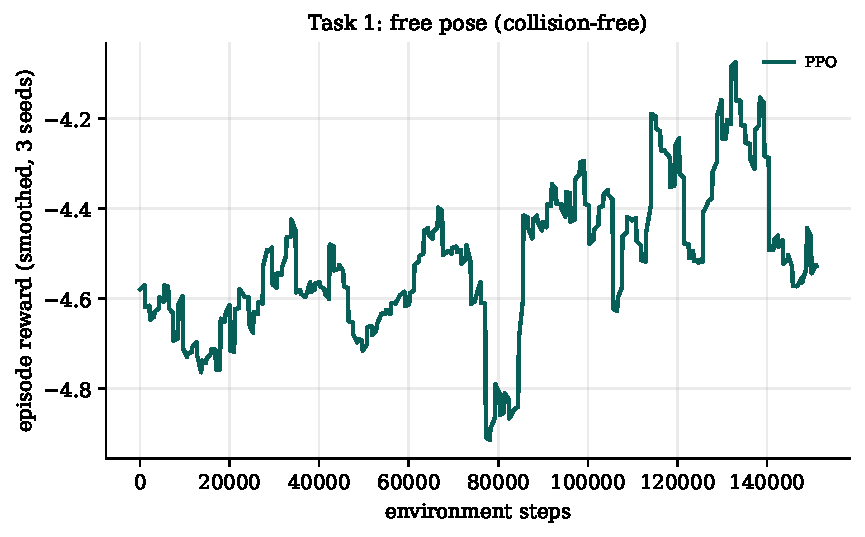
\includegraphics[width=\linewidth]{fig01_learning_free.pdf}
\caption{Task 1 training curves (smoothed success rate vs.\ environment steps; 3 seeds).}\label{fig:learn-free}
\end{figure}

\begin{figure}[!t]\centering
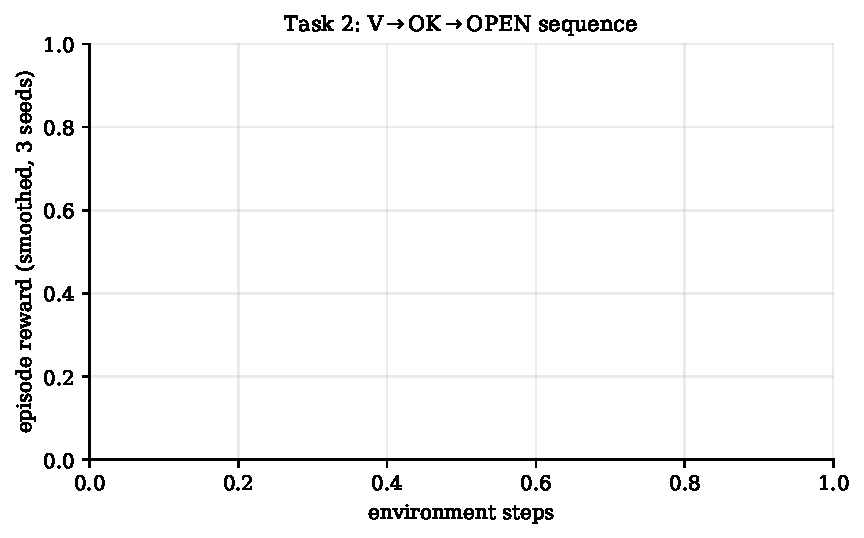
\includegraphics[width=\linewidth]{fig02_learning_seq.pdf}
\caption{Task 2 training curves.}\label{fig:learn-seq}
\end{figure}

\begin{figure}[!t]\centering
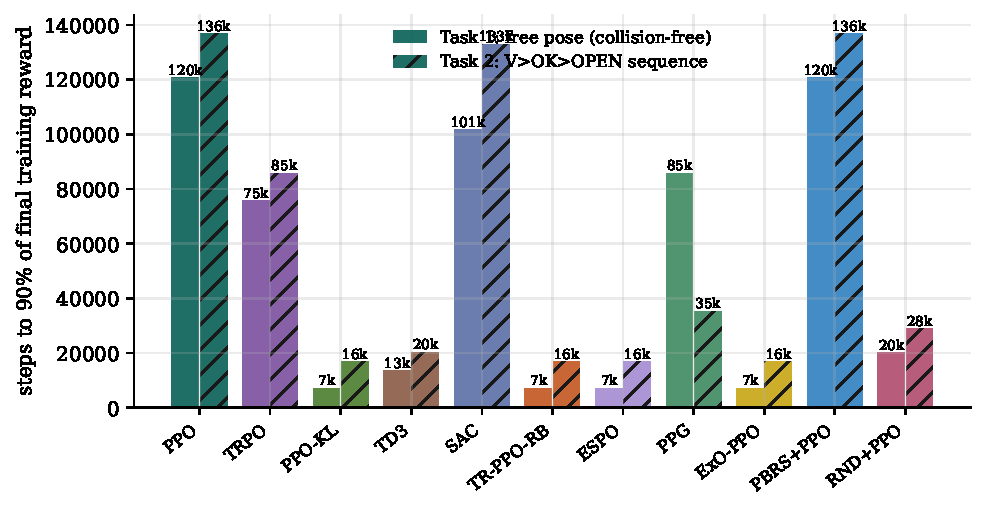
\includegraphics[width=\linewidth]{fig05_sample_efficiency.pdf}
\caption{Sample efficiency: steps for the smoothed training reward to reach 90\% of its final level.}\label{fig:eff}
\end{figure}

\begin{figure}[!t]\centering
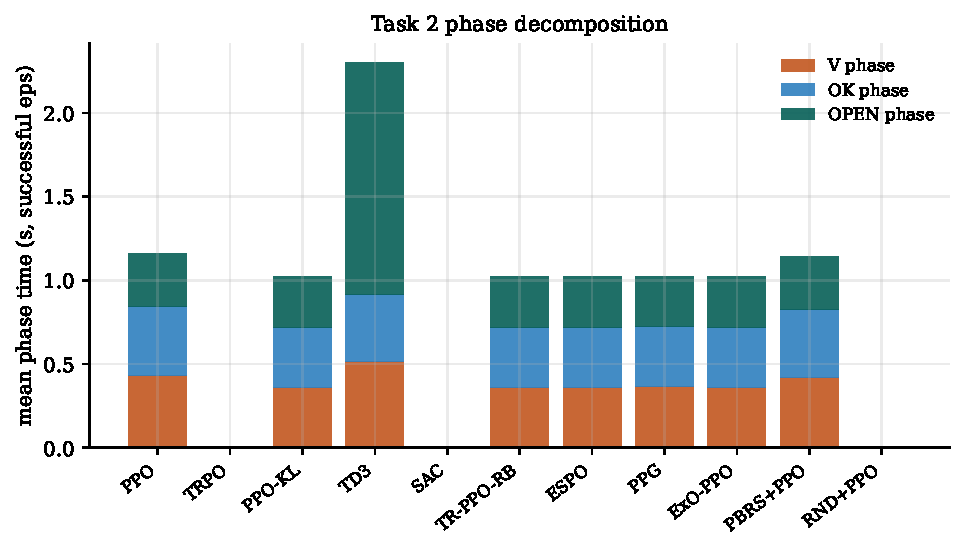
\includegraphics[width=\linewidth]{fig10_phase_decomposition.pdf}
\caption{Task 2 per-phase time decomposition on successful episodes.}\label{fig:phase}
\end{figure}

\begin{figure}[!t]\centering
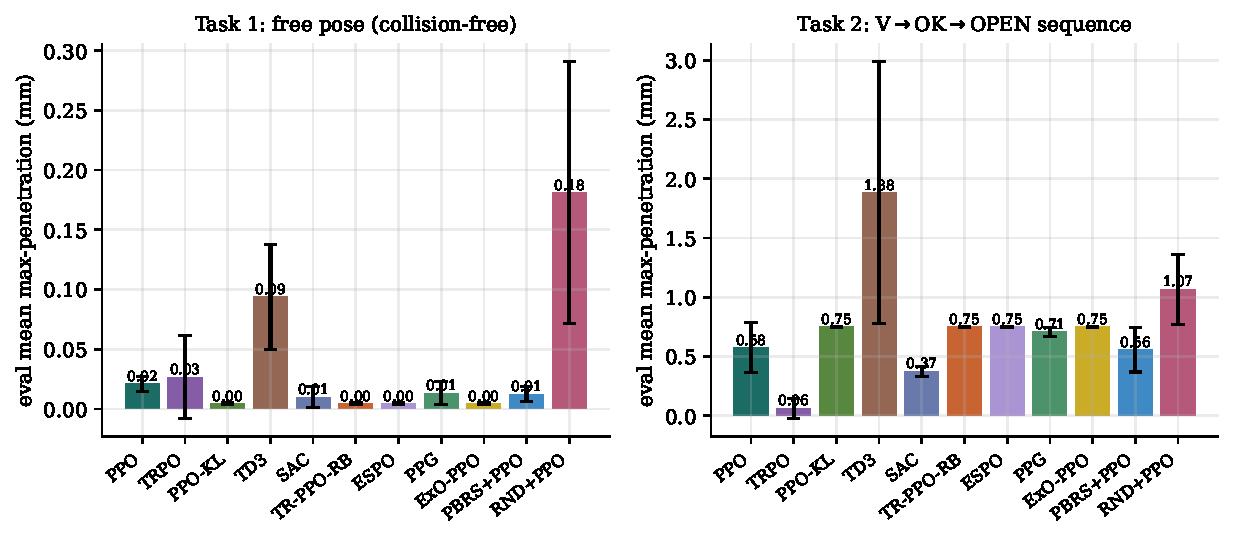
\includegraphics[width=\linewidth]{fig12_safety_penetration.pdf}
\caption{Safety proxy: mean maximum self-penetration during evaluation.}\label{fig:safety}
\end{figure}


\section{Limitations}
Results are simulation-scoped: no claim is made that any trained trajectory
is directly deployable without the separate real-machine pipeline
(rate-limited segmented replay, current/temperature guards, camera
correction). The comparison deliberately fixes one budget; per-method tuning
(e.g., ESPO thresholds, RND $\lambda$, PPG intervals) could reorder method
rankings, and our goal is a controlled, not exhaustive, comparison. PPG's
shared trunk is a capacity change relative to the two-head baseline; we
report it as the published method requires.

\section{Conclusion}
Aitachi-Hand turns an open dexterous hand into a reproducible research
instrument: measured hardware tables, a guarded servo protocol, two
well-posed gesture tasks, and a nine-method controlled study with disclosed
deviations. The platform is released with a four-language report, 12
comparison figures, a textbook, and one-command reproduction scripts.

\begin{thebibliography}{30}\small
\bibitem{orca} ORCA Dexterity, ``ORCA Hand,'' arXiv:2504.04259, 2025; hardware and description repositories, github.com/orcahand.
\bibitem{trpo} J. Schulman et al., ``Trust region policy optimization,'' ICML, 2015.
\bibitem{gae} J. Schulman et al., ``High-dimensional continuous control using generalized advantage estimation,'' ICLR, 2016.
\bibitem{ppo} J. Schulman et al., ``Proximal policy optimization algorithms,'' arXiv:1707.06347, 2017.
\bibitem{impl} L. Engstrom et al., ``Implementation matters in deep RL: A case study on PPO and TRPO,'' ICLR, 2020.
\bibitem{opac} M. Andrychowicz et al., ``What matters in on-policy reinforcement learning? A large-scale empirical study,'' 2021.
\bibitem{trulyp} Truly PPO authors, ``Truly proximal policy optimization,'' 2023 (TR-PPO-RB).
\bibitem{espo} Z. Liu et al., ``ESPO: Early stopping policy optimization,'' 2022.
\bibitem{ppg} K. Cobbe et al., ``Phasic policy gradient,'' ICML, 2021.
\bibitem{exo} ExO-PPO authors, ``Extended off-policy proximal optimization,'' 2025.
\bibitem{oppo} OPPO authors, ``Overlapped generation and scoring for PPO training,'' 2025.
\bibitem{pbrs} A. Y. Ng, D. Harada, and S. Russell, ``Policy invariance under reward transformations,'' ICML, 1999.
\bibitem{pref} P. Christiano et al., ``Deep reinforcement learning from human preferences,'' NeurIPS, 2017.
\bibitem{rnd} Y. Burda et al., ``Exploration by random network distillation,'' ICLR, 2019.
\bibitem{eureka} Y. Ma et al., ``Eureka: Human-level reward design via coding LLMs,'' ICLR, 2024.
\bibitem{twtl} Delayed-rewards TWTL authors, ``TWTL-based reward shaping with policy mixing,'' 2023.
\bibitem{imprm} Improving reward models authors, ``Proximal-preference exploration for reward-model data,'' 2024.
\bibitem{td3} S. Fujimoto, H. van Hoof, and D. Meger, ``Addressing function approximation error in actor-critic methods,'' ICML, 2018.
\bibitem{sac} T. Haarnoja et al., ``Soft actor-critic: Off-policy maximum entropy deep RL with a stochastic actor,'' ICML, 2018.
\bibitem{anymal} ANYmal sim-to-real authors, ``Learning agile and dynamic motor skills for legged robots,'' Science Robotics, 2019.
\bibitem{rma} A. Kumar et al., ``RMA: Rapid motor adaptation,'' CoRL, 2021.
\bibitem{rl100} RL-100 authors, ``Real-time diffusion-policy RL with consistency distillation,'' 2024.
\end{thebibliography}

\end{document}
